\documentclass{beamer}

\usepackage[T1]{fontenc}
\usepackage{inputenc}

\usepackage{amsmath}
\usepackage{listings}
\lstset{
  basicstyle=\footnotesize,
  language=Caml,
  showstringspaces=false,
}


\usetheme{Boadilla}
\usecolortheme{dolphin}
\useoutertheme{infolines}


\setbeamertemplate{footline}
{
  \leavevmode%
  \hbox{%
  \begin{beamercolorbox}[wd=.333333\paperwidth,ht=2.25ex,dp=1ex,center]{author in head/foot}%
    \usebeamerfont{author in head/foot}\insertshortauthor%~~\beamer@ifempty{\insertshortinstitute}{}{(\insertshortinstitute)}
  \end{beamercolorbox}%
  \begin{beamercolorbox}[wd=.333333\paperwidth,ht=2.25ex,dp=1ex,center]{title in head/foot}%
    \usebeamerfont{title in head/foot}\insertshorttitle
  \end{beamercolorbox}%
  \begin{beamercolorbox}[wd=.333333\paperwidth,ht=2.25ex,dp=1ex,right]{date in head/foot}%
    \usebeamerfont{date in head/foot}\insertshortdate{}\hspace*{2em}
    \insertframenumber{} / \inserttotalframenumber\hspace*{2ex}
  \end{beamercolorbox}}%
  \vskip0pt%
}

\title{Cyber security in the Smart Grid: Survey and challenges [WangL14]}
\author{Maxime Puys}
\date{\today}

\graphicspath{{assets/}}

\begin{document}

\begin{frame}
    \maketitle
\end{frame}

\begin{frame}
    \frametitle{Smart Grid}

    \begin{itemize}
        \item Next generation power supply.
            \vfill
        \item Integrates power supply network (e.g.: power lines),
            \vfill
        \item {\bf AND} network communications between parts of the system.
    \end{itemize}
    \vfill
    \begin{figure}[htb]
        \centering
        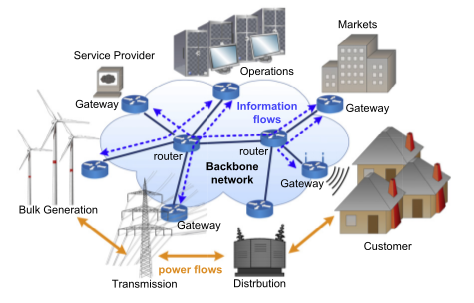
\includegraphics[scale=.6]{smart-grid}
    \end{figure}
\end{frame}

\begin{frame}
    \frametitle{Security requirements}

    Authors analysed security requirements for Smart Grid (also matching most SCADA systems):
    \vfill
    \begin{itemize}
        \item {\bf Availability}
        \vfill
        \item {\bf Integrity}
        \vfill
        \item Confidentiality
    \end{itemize}
    \vfill
    \begin{figure}[htb]
        \centering
        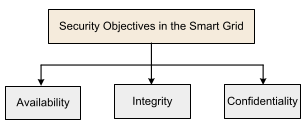
\includegraphics[scale=.6]{objectives}
    \end{figure}
\end{frame}



\section{Availability}

\begin{frame}
    \tableofcontents
\end{frame}

\begin{frame}
    \frametitle{Definition}

    \begin{block}{Availability}
        Ensuring timely and reliable access to and use of information.\\
        \medskip
        {\bf Note:} Authors emphasized the possibility of time-criticity in communications (e.g.: legacy serial modbus).
    \end{block}
    \vfill
    \begin{block}{Risk}
        Disruption of access to or use of information can have dire consequenses such as an electricity blackout or even cause severe damages to infrastructures.\\
        \medskip
        {\bf Note:} Shall the ARAMIS module block packets or just raise alerts ?
    \end{block}
\end{frame}

\begin{frame}
    \frametitle{Attacks on }

    \begin{block}{Denial Of Service}
        Attempt to delay or block communication between entities.
    \end{block}
    \vfill
    Several layers can be attacked:
    \begin{itemize}
        \item Physical layer,
        \item MAC layer,
        \item Network and transport layer,
        \item Application layer.
    \end{itemize}
    \vfill
    {\bf Note:} An adversary does not always need to completly shutdown the trafic but can just delay time-critical messages.
\end{frame}

\begin{frame}
    \frametitle{Physical layer}

    \begin{block}{Channel jamming}
        {\em Brouillage de signal}$_{fr}$ -- Especially for wireless communications.\\
        \medskip
        Mostly happens in local area networks due to range limitations.
    \end{block}
\end{frame}

\begin{frame}
    \frametitle{MAC layer}

    \begin{block}{Compromized backoff parameters}
        An adversary (such as a compromized device) can modify at MAC level parameters (such as Clear Channel Assessment threshold or other parameters in CSMA/CA protocols).\\
        \medskip
        This might cause the medium to ignore other users.
    \end{block}
    \vfill
    \begin{block}{MAC spoofing}
        Address mascarading can help sending fake informations to other devices (e.g.: forged packets) through misconfigured access lists.
    \end{block}
\end{frame}

\begin{frame}
    \frametitle{Network and transport layer}

    \begin{block}{Trafic flooding}
        ICMP flood, SYN flood, teardrops attacks.\\
        \medskip
        Usualy quickly fixed but as SCADA involves quite some legacy devices, it can be a concern.
    \end{block}
    \vfill
    \begin{block}{SCADA example}
        A recent study investigated the impact of a {\bf buffer-flooding attack} on the {\bf DNP3-based SCADA network} with real SCADA system hardware and software, and showed that current SCADA system is quite vulnerable to the DoS attack.
    \end{block}
\end{frame}

\begin{frame}
    \frametitle{Application layer}

    \begin{block}{Attacks}
        Rather than focus on transmission bandwidth, such attacks intend to exhaust ressources of a computer.\\
        \medskip
        {\bf Note:} For example, the ARM/FPGA of the ARAMIS module could be targeted using programming mistakes due to its limited ressources.\\
        \medskip
        {\bf Note 2:} Complexity attacks.
    \end{block}
\end{frame}

\begin{frame}
    \frametitle{Counter-measures}

    \begin{block}{Detection}
        Measuring the Recieved Signal Strength Information (RSSI) can detect jamming attacks.\\
        Packet based detections can be performed at every layer to measure a significant increase of packet transmission failures.\\
        \medskip
        Lot of dedicated softwares (why not {\bf netstat}).
    \end{block}
    \vfill
    \begin{block}{Mitigation}
        Rate limiting policies in routers.\\
        Packets filtering (e.g.: firewalls).\\
        Network reconfiguration: Modify the network topology in order to either add more ressources to the victime or to isolate the attack source. (Does not seems to be applicable to ARAMIS).
    \end{block}
\end{frame}

\section{Integrity}

\begin{frame}
    \tableofcontents[currentsection]
\end{frame}

\begin{frame}
    \frametitle{Definition}

    \begin{block}{Integrity}
        Guarding against improper information modification or destruction is to ensure information nonrepudiation and authenticity.
    \end{block}
    \vfill
    \begin{block}{Risk}
        A loss of integrity (unauthorized modification or destruction of information) can induce incorrect decision regarding machines.
    \end{block}
\end{frame}

\begin{frame}
    \frametitle{Attacks on }

    \begin{block}{Integrity}
        Either {\bf modifying existant information}\\
        \medskip
        Or {\bf inject new forged information}.
    \end{block}
    \vfill
    Both are called {\bf false data injection} in the article.
    \vfill
    {\bf Objective:} Most of time, impact the state estimation and induce operators into making bad decisions.
    \vfill
    In the case of Smart Grid, such attack could be use to impact the electric market and cause potential financial losses.
\end{frame}

\begin{frame}
    \frametitle{Counter-measures}

    \begin{block}{Detection}
        Cryptographic signatures.\\
        \medskip
        Depending on the hardware, potential efficiency problems (regarding to {\bf availability} property).
        HMAC or PKI signatures -> Key management.
    \end{block}
    \vfill
    \begin{block}{Mitigation}
        (Not in the article) -- Error correcting codes.
    \end{block}
\end{frame}

\section{Confidentiality}

\begin{frame}
    \tableofcontents[currentsection]
\end{frame}

\begin{frame}
    \frametitle{Definition}

    \begin{block}{Confidentiality}
         Preserving authorized restrictions on information access and disclosure, mainly to protect personal privacy and proprietary information.
    \end{block}
    \vfill
    \begin{block}{Risk}
        Often said less critical than {\bf availability} and {\bf integrity}.\\
        \medskip
        Becomes crucial when dealing with customers data.
    \end{block}
\end{frame}

\begin{frame}
    \frametitle{Attacks on }

    \begin{block}{Wiretapping}
        {\em \'Ecoutes}$_{fr}$ -- Access to packets contents.
    \end{block}
    \vfill
    \begin{block}{Trafic analyzing}
        Only network topology and flows but not packets contents (?).
    \end{block}
\end{frame}

\begin{frame}
    \frametitle{Counter-measures}

    \begin{block}{Detection}
        ??? -- To my knowledge, it is not possible to detect a sniffer on a network not using any secure protocol.\\
        If yes, how router would be handle ?
    \end{block}
    \vfill
    \begin{block}{Mitigation}
        Cryptographic encryption.\\
        \medskip
        Depending on the hardware, one might choose symetric or PK-encryption.\\
        Hybrid solution such as key exchange using PK-encryption and then symetric with the shared key.\\
        In simple words, using as much as possible secured protocols such as SSH or TLS.
    \end{block}
\end{frame}

\section{Conclusion}

\begin{frame}
    \frametitle{Other security requirements}

    \begin{block}{Attack detection and self-healing}
        Being able to detect an attack and enter some healing mode in order to regain a stable state.
    \end{block}
    \vfill
    \begin{block}{Identification and authentification}
        Identification -- link a virtual entity to a real entity (1 against N).\\
        \medskip
        Authentification -- check if a virtual entity is linked to a real entity (1 against 1).\\
        \medskip
        Question of broadcast and multicast !
    \end{block}
\end{frame}

\begin{frame}
    \frametitle{Other security requirements}

    \begin{block}{Not in the paper}
        Anonymisation -- Whend dealing with custommer\\
        \medskip
        Tracability -- Being able to link a message with its sender and receiver(s).\\
        \medskip
        Non-repudiation -- A user cannot deny that he has sent or recieved a message\\
        \medskip
        Replay attacks -- What happens if a message is sent mote than one time ?\\
        \medskip
        ...
    \end{block}
\end{frame}

\begin{frame}
    \frametitle{Conclusion}

    \begin{center}
        Thanks for your attention!
    \end{center}
\end{frame}

\end{document}
